\documentclass[14pt]{extreport}
\usepackage{gost}
\usepackage{lscape}
\usepackage{multirow}
% объявляем новую команду для переноса строки внутри ячейки таблицы
\newcommand{\specialcell}[2][c]{%
  \begin{tabular}[#1]{@{}c@{}}#2\end{tabular}}



\begin{document}
\begin{figure}[]
		
\includegraphics[scale=0.66]{itmo_image.png}
		\label{pic1}
\end{figure}
\begin{flushleft}
\begin{tabular}{ p{9cm}p{8cm} }
 Группа: K3120 & К работе допущен: \\ 
 Студент: Скворцов И.В. & Работа выполнена: \\  
 Преподаватель: Попов А. С. & Отчет принят: \\    
\end{tabular}
\end{flushleft}

\begin{center}
\Large\textbf{Рабочий протокол и отчёт по\\лабораторной работе №1.04}

\large\textbf{Исследование равноускоренного вращательного движения \\ (маятник Обербека)}
\end{center}

\section*{1. Цель работы.}

\begin{enumerate}
    \item Проверить основной закон динамики вращений.
    \item Проверить зависимость момента инерции от положения масс относительно оси вращения.
\end{enumerate}

\section*{2. Задачи.}
\begin{enumerate}
    \item Измерить время падения груза при разной массе груза и разном положении утяжелителей на крестовине.
    \item Расчет ускорение груза, углового ускорения крестовины и моменты сила натяжения нити. 
    \item Расчет момента инерции крестовины с утяжелителями и момента силы трения. 
    \item Исследование зависимости момента силы натяжения нити от углового ускорения. Проверка основного закона динамики вращения.
    \item Исследование зависимости момента инерции от положения масс относительно оси вращения. Проверка теоремы Штейнера. 
\end{enumerate}

\section*{3. Объект исследования}
Равноускоренное вращательное движение маятника Обербека.

\section*{4. Метод экспериментального исследования.}
Эмпирический лабораторный экспериментальный

\section*{5. Рабочие формулы и исходные данные.}
Ускорение груза:
\begin{equation}\label{f1}
    a = \frac{2*h}{t^2}
\end{equation}

Ускорение крестовины:
\begin{equation}\label{f1}
    \varepsilon = \frac{2*a}{d}
\end{equation}

Сила натяжения нити:
\begin{equation}\label{f1}
    T = m(g - a)
\end{equation}

Момент силы натяжения нити:
\begin{equation}\label{f1}
    M = \frac{md}{2}(g - a)
\end{equation}

Основной закон динамики вращения крестовины:
\begin{equation}\label{f1}
    I\varepsilon = M - M_{Tp}
\end{equation}

Момент инерции крестовины:
\begin{equation}\label{f1}
    I = I_{0} + 4m_{YT}R^2
\end{equation}

Расстояние между осью вращения и центром утяжелителя:
\begin{equation}\label{f1}
    R = l_{1} + (n-1)l_{0} + 0.5b
\end{equation}

\section*{6. Измерительные приборы}
\begin{table}[H]\label{t1}
\caption{Измерительные приборы.}
\centering
\begin{tabular}{|c|c|c|c|c|}
\hline
 № и/п & Наименование & Тип прибора & Используемый & Погрешность \\ 
 & & & диапазон & прибора \\ \hline
 1 & Линейка на вертикали & Цифровой & [0; 700], мм & 0.5, мм \\ \hline
 2 & Секундомер цифровой & Цифровой & [0; 60], с & 0.0005, с \\ \hline
 
\end{tabular}
\end{table}

\section*{7. Схема установки}
\begin{figure}[H]
	\begin{center}
		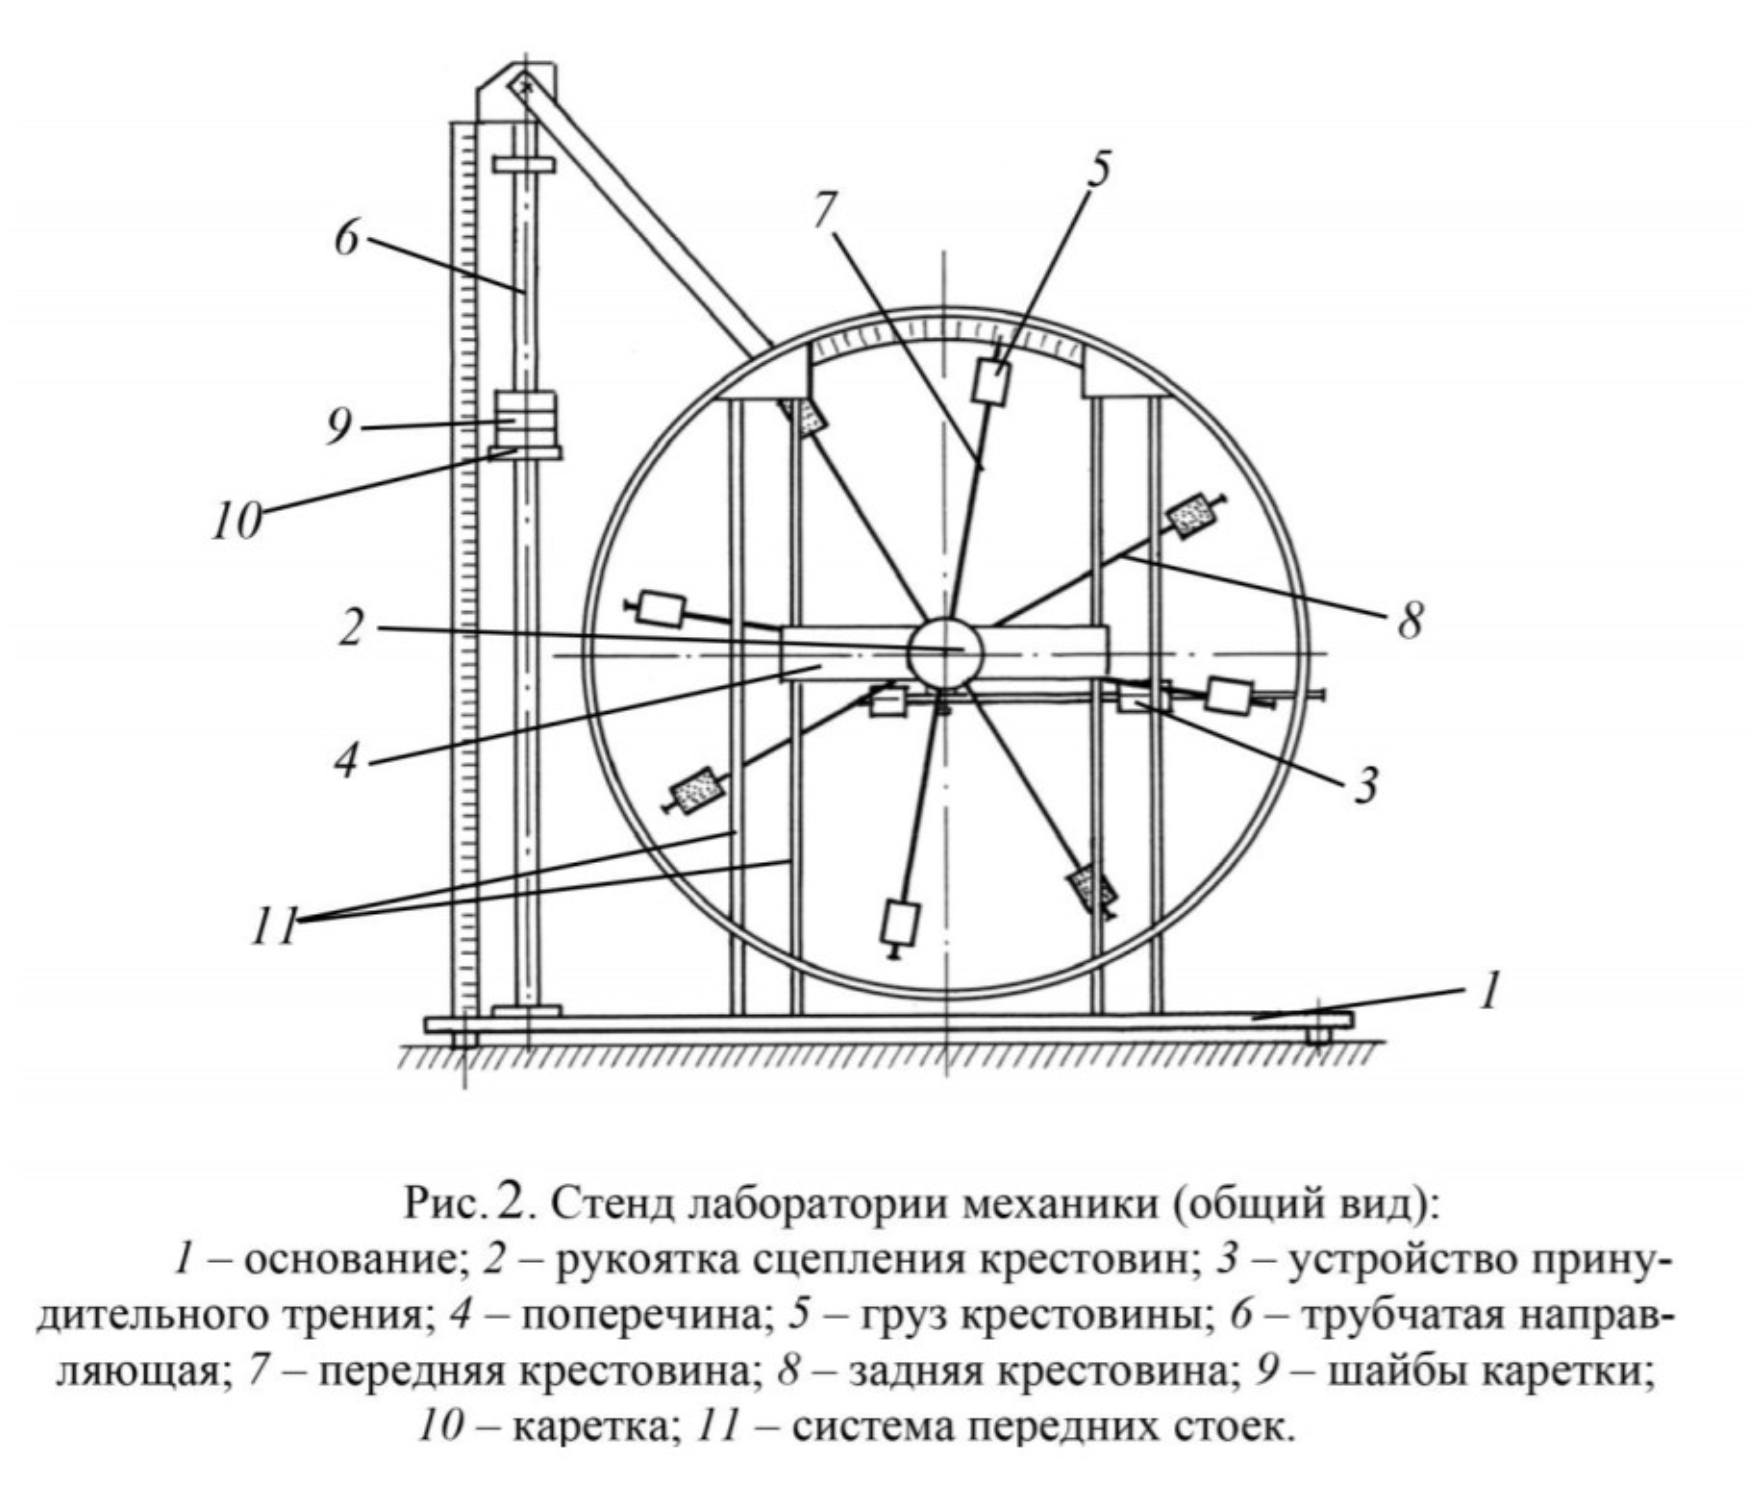
\includegraphics[scale=0.5]{scheme.png}
		\caption{Схема экспериментальной установки}
		\label{pic}
	\end{center}
\end{figure}

\newpage
\section*{8. Результаты прямых измерений и их обработка.}
\begin{table}[H]
    \centering
    \begin{tabular}{|c|c|c|c|c|c|c|}
    \hline
         \multirow{2}{*}{\specialcell{Масса \\ груза, г}} & \multicolumn{6}{c|}{Положение утяжелителя} \\
         \cline{2-7}
         & 1 риска & 2 риска & 3 риска & 4 риска & 5 риска & 6 риска \\ \hline
         \multirow{4}{*}{$267.0 \pm 1.0 $} &  4.522 & 5.339	&6.152	&7.275	&8.184&	11.587\\ \cline{2-7}
         &4.673	&5.289&	6.303&	7.118&	7.269&	12.152\\ \cline{2-7}
         & 4.779 &	5.133 &	6.252&	6.814	&8.385	&9.917\\ \cline{2-7}
         & 4.658 &	5.25367 &	6.23567&	7.069&	7.946	&11.21867\\ \hline
         \multirow{4}{*}{$487.0 \pm 1.5 $} &  3.001	&3.864&	4.522	&4.884&	6.408&	6.867\\ \cline{2-7}
         & 3.509	&3.813&	4.728	&5.084	&6.458&	6.712\\ \cline{2-7}
         & 3.505	&3.711	&4.678	&5.184	&5.847	&6.73\\ \cline{2-7}
         & 3.3383 &3.796	&4.64267&	5.05067&	6.23767&	6.76967\\ \hline
         \multirow{4}{*}{$707.0 \pm 2.0 $} & 2.593&	3.204&	3.712&	4.168&	4.676&	5.591\\ \cline{2-7}
         & 2.643&	3.155&	3.41&	3.916&	4.879&	5.562 \\ \cline{2-7}
         & 2.545&	3.053&	3.505&	4.526&	4.625&	5.543 \\ \cline{2-7}
         &2.59367&	3.1373&	3.5423&	4.203&	4.7267&	5.5653 \\ \hline
         \multirow{4}{*}{$927.0 \pm 2.5 $} & 2.136&	2.593&	3.559&	3.456&	4.173&	4.473\\ \cline{2 - 7}
&2.137&	2.594&	3.203&	3.51&	4.17&	4.83 \\ \cline{2 -7}
&2.135&	2.492&	3.001&	3.459&	4.218&	4.47 \\ \cline{2-7}
&2.136&	2.55967&	3.254&	3.475&	4.187&	4.591 \\ \hline
         
    \end{tabular}
    \caption{ Протокол измерений времени падения груза при разной массе груза и разном положении утяжелителей на крестовине}
    \label{tab:my_label}
\end{table}

\section*{9. Расчет результатов косвенных измерений.}

1) Пример вычисления значения $t_{cp}$ для 1 риски и массы груза 267г:\\
\begin{center}
$t_{cp} = \frac{4.522 + 4.673 + 4.779}{3} = (4.658)\text{, c}$ \\
\end{center}

2) $\Delta t$ для первого значения $t_{cp}$: \\
\begin{center}
    $\Delta t = 0.321 \textbf{, с}$
\end{center}

3) Рассчитаем ускорение $\alpha$, угловое ускорение $\varepsilon$ и момента $M$ силы натяжения нити.

\begin{table}[!ht]
    \centering
    \begin{tabular}{|l|l|l|l|l|l|l|}
    \hline
        $\alpha \text{, м/}c^2$ & 1 риска & 2 риска & 3 риска & 4 риска & 5 риска & 6 риска  \\ \hline
        1 груз & 0.0645251 & 0.0507227 & 0.0360049 & 0.0280163 & 0.022173 & 0.011123 \\ \hline
        2 груза & 0.1256228 & 0.097157343 & 0.0649520 & 0.0548820 & 0.03598 & 0.030548  \\ \hline
        3 груза & 0.2081132 & 0.1422350 & 0.111570 & 0.0792392 & 0.06266 & 0.045200 \\ \hline
        4 груза & 0.3068495 & 0.2136786 & 0.1322187 & 0.1159360 & 0.0798586 & 0.066422\\ \hline
    \end{tabular}
    \caption{Значение $\alpha$ ускорение груза}
\end{table}

\begin{table}[!ht]
    \centering
    \begin{tabular}{|l|l|l|l|l|l|l|}
    \hline
        $\varepsilon \text{, рад/$c^2$}$ & 1 риска & 2 риска & 3 риска & 4 риска & 5 риска & 6 риска  \\ \hline
        1 груз & 2.805441 & 2.205338 & 1.565432755 & 1.218103627 & 0.964057 & 0.48363  \\ \hline
        2 груз & 5.461862 & 4.224232 & 2.824003255 & 2.386177717 & 1.564429 & 1.32820 \\ \hline
        3 груз & 9.048401 & 6.184133 & 4.850889122 & 3.445184907 & 2.724521 & 1.96525 \\ \hline
        4 груз & 13.34128 & 9.290377 & 5.748639868 & 5.040696876 & 3.472116 & 2.88792 \\ \hline
    \end{tabular}
    \caption{Значение $\varepsilon$ углового ускорения}
\end{table}

\begin{table}[!ht]
    \centering
    \begin{tabular}{|l|l|l|l|l|l|l|}
    \hline
        M, Н*м & 1 риска & 2 риска & 3 риска & 4 риска & 5 риска & 6 риска  \\ \hline
        1 груз & 0.0597855 & 0.059870311 & 0.0599606 & 0.0600097 & 0.060045 & 0.060113  \\ \hline
        2 груз & 0.1083626 & 0.108681541 & 0.1090422 & 0.1091550 & 0.109367 & 0.109427 \\ \hline
        3 груз & 0.1559736 & 0.157044915 & 0.1575435 & 0.1580692 & 0.158338& 0.158622 \\ \hline
        4 груз & 0.2024037 & 0.204389957 & 0.2061267 & 0.2064739 & 0.207243 & 0.207529 \\ \hline
    \end{tabular}
    \caption{Значение $M$ момента сила натяжения нити}
\end{table}

4) Рассчитаем погрешность для первых значений $\varepsilon, \alpha, M$:
\begin{center}
    $\Delta a = 0.00087\text{, м/}c^2\quad \varepsilon_{a} = 1.35\%\quad \alpha = 0.95$\\
    $\Delta \varepsilon = 0.0943\text{, рад/}c^2\quad \varepsilon_{\varepsilon} = 3.37\%\quad \alpha = 0.95$\\
    $\Delta M = 0.00068\text{, Н*м}\quad \varepsilon_{M} = 1.1\%\quad \alpha = 0.95$\\
\end{center}

5) С помощью метода наименьших квадратов вычислим момент I инерции крестовины с утяжелителями и момент силы трения $M_{Tp}$ для каждого положения утяжелителя.
\newpage
\begin{table}[!ht]
    \centering
    \begin{tabular}{|l|l|l|l|l|l|l|}
    \hline
        ~ & 1 риска & 2 риска & 3 риска & 4 риска & 5 риска & 6 риска  \\ \hline
        $M_{Tp}$ & 0.0293 &0.0204 &0.0104 &0.0166 &0.0122 &0.0121\\ \hline
        $I$ & ~0.0133 &0.0204 &0.0327 &0.0386 &0.0557 &0.0558 \\ \hline
    \end{tabular}
    \caption{Значения $M_{Tp}$ и I, полученные с помощью МНК}
\end{table}

6) Посчитаем $R^2$ и занесем в таблицу.

\begin{table}[!ht]
    \centering
    \begin{tabular}{|l|l|l|l|l|l|l|}
    \hline
        ~ & 1 риска & 2 риска & 3 риска & 4 риска & 5 риска & 6 риска  \\ \hline
        R & 0.0485 & 0.0735 & 0.086 & 0.0985 & 0.111 & 0.1235  \\ \hline
        Rˆ2 & 0.002352 & 0.005402 & 0.0073 & 0.009702 & 0.0123 & 0.015252  \\ \hline
        I & 0.013350 & 0.0204633 & 0.0327528 & 0.0386421 & 0.0557029 & 0.0558086 \\ \hline
    \end{tabular}
    \caption{Таблица со значениями $R, R^2, I$}
\end{table}

7) На основе вышеприведенных данных, с помощью мнк найдем $m_{YT}$ и $I_0$ из зависимости $I = I_0 + 4m_{YT}R^2$. Посчитаем их погрешность.
\begin{center}
    $m_{YT} = 0.9175 \text{, кг}$ \\
    $\Delta m_{yt} = 0.5S_b = 0.206 \text{, кг} \quad \epsilon_{m_{YT}} = 22\%$ \\
    $I_0 = 0.0041 \text{, Н*м} $ \\
    $\Delta I_0 = 2S_a = 0.000802 \text{, Н*м} \quad \epsilon_{I_0} = 19.6\%$
\end{center}

\section*{10. Графики}
\begin{figure}[H]
	\begin{center}
		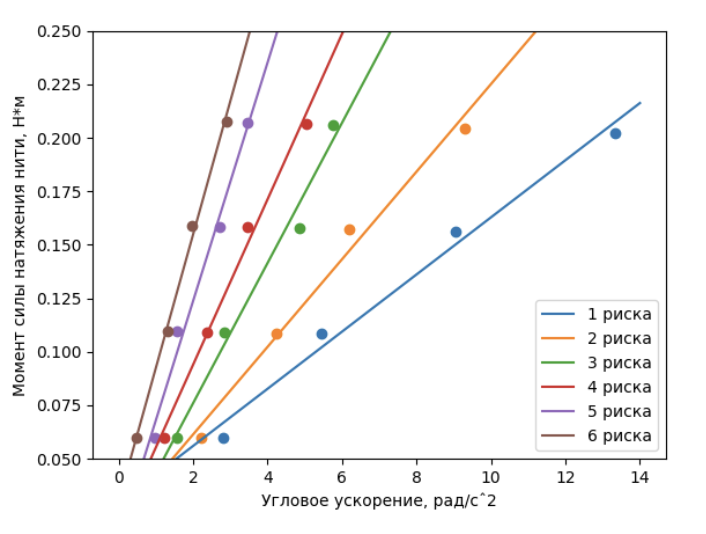
\includegraphics[scale=1]{M_e.png}
		\caption{График зависимости $M(\varepsilon)$}
		\label{pic}
	\end{center}
\end{figure}

\begin{figure}[H]
	\begin{center}
		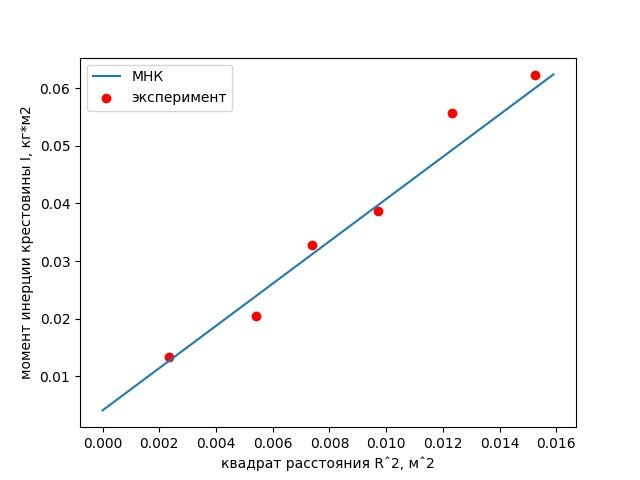
\includegraphics[scale=0.55]{I_R_2.jpg}
		\caption{График зависимости $I(R^2)$}
		\label{pic}
	\end{center}
\end{figure}

\section*{11. Окончательные результаты}

\begin{center}
    $\alpha = (0.0645 \pm 0.0009)\text{ м/$c^2$;}\quad \varepsilon_{\alpha} = 1.35\%\text{;} \quad \alpha = 0.95\text{.}$ \\
    $\varepsilon = (2.81 \pm 0.09)\text{ рад/$c^2$;}\quad \varepsilon_{\varepsilon} = 3.37\%\text{;} \quad \alpha = 0.95\text{.}$ \\
    $M = (0.0598 \pm 0.0007)\text{ Н*м;}\quad \varepsilon_{M} = 1.1\%\text{;} \quad \alpha = 0.95\text{.}$\\\
    
    $m_{YT} = (0.92 \pm 0.21)\text{ кг;}\quad \varepsilon_{m_{YT}} = 22\%\text{;} \quad \alpha = 0.95\text{.}$
    $I_0 = (0.0041 \pm 0.0008)\text{ кг*мˆ2;}\quad \varepsilon_{I_0} = 19.6\%\text{;} \quad \alpha = 0.95\text{.}$
\end{center}

\section*{12. Выводы и анализ результатов работы}

В ходе лабораторной работы был подвергнут проверке основной закон динамики вращения. Анализ график зависимости $M(\varepsilon)$ позволяет сделать сделать вывод, что зависимость является линейной, полученные экспериментальные значения совпадают с теоретическими в пределах погрешности. Рассматривая график зависимости $I(R^2)$ можно убедиться в предположении, что момент инерции прямо пропорционален квадрату расстояния до утяжелителей.
\end{document}

